% ------------------------------------------------------------------------
% Este documento foi criado com base no abtex2-modelo-trabalho-academico.tex, v-1.9.6 laurocesar - Copyright 2012-2016 by abnTeX2 group at http://www.abntex.net.br/ 
%
% O modelo original, abnTeX2, é um Modelo de Trabalho Academico (tese de doutorado, dissertacao de
% mestrado e trabalhos monograficos em geral) em conformidade com ABNT NBR 14724:2011: Informacao e documentacao - Trabalhos academicos -
% ------------------------------------------------------------------------

\documentclass[
	% -- opções da classe memoir --
	12pt,				% tamanho da fonte
	openright,			% capítulos começam em pág ímpar (insere página vazia caso preciso)
	twoside,			% para impressão em recto e verso. Oposto a oneside
	a4paper,			% tamanho do papel. 
	% -- opções da classe abntex2 --
	%chapter=TITLE,		% títulos de capítulos convertidos em letras maiúsculas
	%section=TITLE,		% títulos de seções convertidos em letras maiúsculas
	%subsection=TITLE,	% títulos de subseções convertidos em letras maiúsculas
	%subsubsection=TITLE,% títulos de subsubseções convertidos em letras maiúsculas
	% -- opções do pacote babel --
	english,			% idioma adicional para hifenização
	french,				% idioma adicional para hifenização
	spanish,			% idioma adicional para hifenização
	brazil,				% o último idioma é o principal do documento
	hyphens
	]{abntex2}

% ---
% Pacotes básicos 
% ---
\usepackage{cmap}					 	   % Mapear caracteres especiais no PDF
\usepackage{lmodern} 					 % Usa a fonte Latin Modern			
\usepackage[T1]{fontenc}				% Selecao de codigos de fonte.
\usepackage[utf8]{inputenc}			   % Codificacao do documento (conversão automática dos acentos)
\usepackage{lastpage}					  % Usado pela Ficha catalográfica
\usepackage{indentfirst}				  % Indenta o primeiro parágrafo de cada seção.
\usepackage{color}							  % Controle das cores
\usepackage{graphicx}					  % Inclusão de gráficos
\usepackage{microtype} 					% para melhorias de justificação
% ---
		
% ---
% Pacotes de citações
% ---
\usepackage{hyperref}
\usepackage[hyphenbreaks]{breakurl}
\usepackage[alf]{abntex2cite}	% Citações padrão ABNT

% ---
% Pacotes para tabela de mais de uma página
% ---
\usepackage{lscape}
\usepackage{longtable}

% ---
% Pacotes para manter a numeracao das notas de rodapé continuas entre capitulos
% ---
\usepackage{chngcntr}
\counterwithout{footnote}{chapter}

% --- 
% CONFIGURAÇÕES DE PACOTES
% --- 

\RequirePackage{utf_macros} % ajustes para tema da UFT
\RequirePackage{dados_trabalho} % arquivo com dados específicos do trabalho
\RequirePackage{info_code}

\usepackage{todonotes}
\usepackage{soul}
\usepackage[normalem]{ulem}
\usepackage{xcolor}
\usepackage{amsmath,amsfonts,amssymb} % pacote matematico
\usepackage{mathptmx} % fonte times
\usepackage{url}
\usepackage{caption}
\usepackage{subcaption}
\usepackage{float}
\usepackage{lastpage}
\usepackage{array}
\usepackage{booktabs}
\usepackage{ifthen}

% ---
% Pacotes para utilizar imagens do tipo .eps
% ---
\usepackage{epstopdf}
\DeclareGraphicsExtensions{.eps}

% ---
% Pacotes para ajustar problema das notas de rodapé muito longas
% ---
\usepackage[bottom]{footmisc}
\raggedbottom 
\addtolength{\topskip}{0pt plus 10pt}
\interfootnotelinepenalty=10000

% ---
% Pacotes para evitar linhas orfãs
% ---
\widowpenalty10000
\clubpenalty10000

% Caminho da pasta images
\graphicspath{ {imagens/} }

% ---
% Configurações de aparência do PDF final

% alterando o aspecto da cor azul
\ifthenelse{\equal{\LinkAzul}{S}}
	{\definecolor{blue}{RGB}{41,5,195}} % links azuis
	{\definecolor{blue}{RGB}{0,0,0}}% links pretos

% informações do PDF
\makeatletter
\hypersetup{
     	%pagebackref=true,
		pdftitle={\@title}, 
		pdfauthor={\@author},
    	pdfsubject={\imprimirpreambulo},
	    pdfcreator={LaTeX with abnTeX2},
		pdfkeywords={\PalavrasChave}, 
		colorlinks=true,       		% false: boxed links; true: colored links
    	linkcolor=blue,          	% color of internal links
    	citecolor=blue,        		% color of links to bibliography
    	filecolor=magenta,      		% color of file links
		urlcolor=blue,
		bookmarksdepth=4
}
\makeatother
% --- 

% ---
% compila o indice
% ---
\makeindex
% ---

% ----
% Início do documento
% ----

\begin{document}
\verificaTitulo
% Seleciona o idioma do documento (conforme pacotes do babel)
%\selectlanguage{english}
\selectlanguage{brazil}

% corrigir problema de urls muito longas
\hyphenrules{nohyphenation}\exhyphenpenalty 10000

%corrigir problema dos espaços em branco que forçavam o texto a ficar proximo da imagem
\raggedbottom

% desativa hifenização mantendo o texto justificado.
\tolerance=1
\emergencystretch=\maxdimen
\hyphenpenalty=10000
\hbadness=10000
\sloppy

% Retira espaço extra obsoleto entre as frases.
\frenchspacing 

% ----------------------------------------------------------
% ELEMENTOS PRÉ-TEXTUAIS
% ----------------------------------------------------------
% \pretextual

% ---
% Capa
% ---
\imprimircapa
% ---

% ---
% Folha de rosto
% (o * indica que haverá a ficha bibliográfica)
% ---
\imprimirfolhaderosto
% ---

% ---
% Agradecimentos
% ---
	\ifthenelse{\equal{\ExisteAgradecimentos}{S}}
	{	
		\begin{agradecimentos}
			Texto dos agradecimentos
		\end{agradecimentos}
	}
	{}%
% ---

% ---
% Epígrafe
% ---
	\ifthenelse{\equal{\ExisteEpigrafe}{S}}
	{	
		\begin{epigrafe}
			\vspace*{\fill}	
			\begin{flushright}
				Texto da sua epígrafe
			\end{flushright}
		\end{epigrafe}
	}
	{}% 
%} 

% ---

% ---
% RESUMOS
% ---

% resumo em português
\setlength{\absparsep}{18pt} % ajusta o espaçamento dos parágrafos do resumo
\begin{resumo}
	\NomeCitacao. \MakeUppercase{\TituloCorpo}.  \pageref{LastPage} p. \TipoTrabalho\ – \Programa, \Universidade. \Local, \the\year.
	
	Texto do resumo em português
	
	\textbf{Palavras-chave}: \PalavrasChave
\end{resumo}

% resumo em inglês
\begin{resumo}[Abstract]
	\begin{otherlanguage*}{english}
		\NomeCitacao. \MakeUppercase{\TituloEN}.  \pageref{LastPage} p. \TipoTrabalhoEN\ – \ProgramaEN, \UniversidadeEN. \Local, \the\year.
		
		Texto do resumo em inglês. 

O resumo em língua estrangeira é obrigatório segundo a NBR 6028. Caso o seu resumo seja em língua diferente do inglês, favor consultar a Wiki deste projeto para dicas de como resolver este problema. Link da Wiki ->  \url{https://github.com/pslz/ABNTexUTFPR/wiki}
		
		\textbf{Keywords}: \PalavrasChaveEN
	\end{otherlanguage*}
\end{resumo}

% ---
% inserir lista de ilustrações
% ---
\pdfbookmark[0]{\listfigurename}{lof}
\ifthenelse{\equal{\ExisteFigura}{S}}
{\listoffigures*}
{}%
\cleardoublepage
% ---

% ---
% inserir lista de tabelas
% ---
\pdfbookmark[0]{\listtablename}{lot}
\ifthenelse{\equal{\ExisteTabela}{S}}
{\listoftables*}
{}%
\cleardoublepage
% ---

% ---
% inserir lista de abreviaturas e siglas
% ---
\ifthenelse{\equal{\ExisteSigla}{S}}
{\begin{siglas} \item [CTS] Ciência, Tecnologia e Sociedade \end{siglas}}
{}%
% ---

% ---
% inserir o sumario
% ---
\pdfbookmark[0]{\contentsname}{toc}
\tableofcontents*
\cleardoublepage
% ---



% ----------------------------------------------------------
% ELEMENTOS TEXTUAIS
% ----------------------------------------------------------
\textual

\chapter{Introdução}

Esse é o texto da introdução do capítulo. 

\section{Primeira Seção}

Aqui temos uma seção de segundo nível, ou subseção.

Segundo \citeonline{Dissertacao2012}, o termo xyz refere-se à x coisas e outras mais. Entretanto, há trabalhos que discordam \cite{ArtigoDeCongresso2017}.

Neste sentido, o termo xyz pode ser compreendido, por meio dessa citação direta longa, como

\begin{citacao}
	Essa é uma citação longa falando sobre o termo xyz. Pra ela ficar realmente longa, vou utilizar o Lorem Ipsum. Lorem ipsum dolor sit amet, consectetur adipiscing elit. Nulla neque enim, convallis et rutrum id, euismod at purus. Quisque finibus placerat sapien ut volutpat. Mauris vitae velit a lacus blandit suscipit in at magna. Nulla vel faucibus turpis. Donec in justo condimentum, viverra nibh sed, maximus quam. Nulla facilisi. Suspendisse massa nisi, sollicitudin eu bibendum at, ultrices ut ante. Praesent lobortis dolor at ipsum ultrices porta. Aenean nec congue metus. Vivamus vitae interdum arcu. Fusce pulvinar euismod rhoncus. Vestibulum ultrices, ipsum non porttitor aliquam, nulla augue convallis dui, ultricies imperdiet purus ex eu ipsum. Praesent faucibus congue molestie. Ut odio orci, congue in venenatis a, dapibus vel tortor. Proin fringilla dolor nisi, nec porttitor purus lobortis vitae. Aliquam metus elit, varius eu mauris non, bibendum imperdiet massa. Ao final vou simular uma referência \cite[p.20]{Livro1990}.
\end{citacao}

\subsection{Seção de terceiro nível} \label{sec:outra}

Aqui uma seção de terceiro nível

Agora vamos incluir uma imagem e referenciá-la (Figura \ref{fig:sorvete}).

\begin{figure}[H]
	\centering
	\caption{Sorvete}
	\centering
	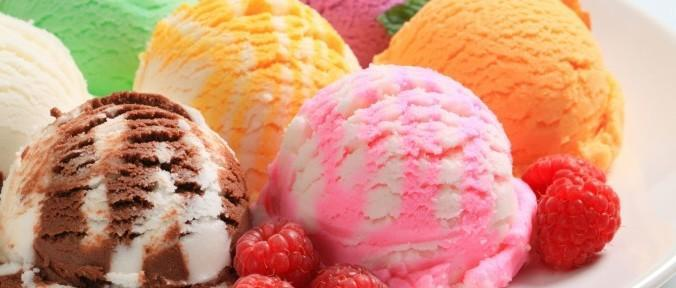
\includegraphics[width=0.7\textwidth]{sorvete.jpg}
	\fonte{\citeonline{Sorvete2017}}
	\label{fig:sorvete}
\end{figure}

\subsubsection{Seção de quarto nível}

Aqui exemplo de uma seção de quarto nível

Abaixo mais um texto com Lorem Ipsum para exemplificar a formatação.

Lorem ipsum dolor sit amet, consectetur adipiscing elit. Nulla neque enim, convallis et rutrum id, euismod at purus. Quisque finibus placerat sapien ut volutpat. Mauris vitae velit a lacus blandit suscipit in at magna. Nulla vel faucibus turpis. Donec in justo condimentum, viverra nibh sed, maximus quam. Nulla facilisi. Suspendisse massa nisi, sollicitudin eu bibendum at, ultrices ut ante. Praesent lobortis dolor at ipsum ultrices porta. Aenean nec congue metus. Vivamus vitae interdum arcu. Fusce pulvinar euismod rhoncus. Vestibulum ultrices, ipsum non porttitor aliquam, nulla augue convallis dui, ultricies imperdiet purus ex eu ipsum. Praesent faucibus congue molestie. Ut odio orci, congue in venenatis a, dapibus vel tortor. Proin fringilla dolor nisi, nec porttitor purus lobortis vitae. Aliquam metus elit, varius eu mauris non, bibendum imperdiet massa.


\chapter{Desenvolvimento}

Texto introdutório do capítulo corrente.

\section{Seção com Exemplo de Tabelas} \label{sec:tabela}

Abaixo o exemplo de uma tabela longa, ou seja, uma tabela que necessite mais de uma página para ser apresentada.

Nossa tabela terá 6 colunas e 10 linhas.

Existem sites que auxiliam na estruturação de tabelas para o LaTeX, como o \textbf{Tables Generator}\footnote{\url{https://www.tablesgenerator.com/}}. Entretanto, não encontrei um gerador de tabelas longas.

O conteúdo dessa tabela é preenchido com Lorem Ipsum apenas para exemplo.

\renewcommand*{\arraystretch}{1.5}

{\footnotesize
	\centering
	\begin{longtable}{ M{.10\textwidth}  M{.15\textwidth}  M{.16\textwidth}  M{.15\textwidth}  M{.16\textwidth}  M{.12\textwidth} }
		
		\caption{Título da Tabela Longa} \\ \toprule
		\label{tabela:longa}
		
		\textbf{Coluna 1} & \textbf{Coluna 2} & \textbf{Coluna 3} & \textbf{Coluna 4} & \textbf{Coluna 5} & \textbf{Coluna 6} \\ % Note a separação de col. e a quebra de linhas
		
		\hline 
		
		\endfirsthead
		& & & & & \null \hfill(conclusão)\\ 
		
		\toprule
		
		\textbf{Coluna 1} & \textbf{Coluna 2} & \textbf{Coluna 3} & \textbf{Coluna 4} & \textbf{Coluna 5} & \textbf{Coluna 6} \\ %
		
		\hline % para uma linha horizontal
		
		\endhead
		
		Linha 01 & Lorem ipsum dolor sit amet, consectetur adipiscing elit. & Nulla neque enim, convallis et rutrum id, euismod at purus. &  Quisque finibus placerat sapien ut volutpat.  & Mauris vitae velit a lacus blandit suscipit in at magna. Nulla vel faucibus turpis. Donec in justo condimentum, viverra nibh sed, maximus quam. & Nulla facilisi. \\
		
		Linha 02 & Suspendisse massa nisi, sollicitudin eu bibendum at, ultrices ut ante. & Praesent lobortis dolor at ipsum ultrices porta &  Porchetta & Aenean nec congue metus & Vivamus vitae interdum arcu \\
		
		Linha 03 & Fusce pulvinar euismod rhoncus & Vestibulum ultrices, ipsum non porttitor aliquam, nulla augue convallis dui, ultricies imperdiet purus ex eu ipsum &  Praesent faucibus congue molestie & Ut odio orci, congue in venenatis a, dapibus vel tortor & Proin fringilla dolor nisi, nec porttitor purus lobortis vitae \\
		
		Linha 04 & Aliquam metus elit, varius eu mauris non, bibendum imperdiet massa & Suspendisse est libero, lacinia nec odio quis, lobortis accumsan tortor &  Lorem ipsum dolor sit amet & Morbi mauris neque, porta at condimentum in, tempor id lacus & In ut risus arcu \\
		
		Linha 05 & Vestibulum eleifend non augue consectetur consectetur & Nam auctor vitae ipsum eu iaculis &  Porchetta & Curabitur consectetur & Nam dignissim accumsan eleifend \\
		
		Linha 06 & Nam vitae convallis ante & Duis at nunc et ligula fermentum pharetra &  Vestibulum ante ipsum primis in faucibus orci luctus et ultrices posuere cubilia Curae & Sed auctor purus quis sodales rutrum & Sed imperdiet euismod tellus \\
		
		Linha 07 & Duis eu nulla ipsum & Nulla quis volutpat nisi, at aliquam quam &  Aliquam porttitor suscipit diam a sagittis & Duis auctor interdum ipsum eu bibendum & Sed eu velit magna \\
		
		Linha 08 & Quisque vel odio nisi & Nam ac ante enim &  Integer porttitor sollicitudin convallis & Sed cursus velit quis feugiat facilisis & Suspendisse volutpat in massa quis aliquam \\
		
		Linha 09 & Donec sit amet enim quis lorem interdum imperdiet & Suspendisse bibendum, nunc sed ultrices tristique, tellus odio aliquam neque, ut venenatis ipsum velit et lorem &  Fusce eget lorem ut enim rutrum tristique & Sed volutpat nunc at sodales mollis & Nunc tincidunt \\
		
		Linha 10 & Interdum et malesuada fames ac ante ipsum primis in faucibus & Aliquam pharetra, tortor in semper porta &  Sed porttitor neque non lacus laoreet iaculis. & Pellentesque accumsan vulputate pharetra & Aliquam et velit dui \\ \toprule
		
		% não é preciso quebrar a última linha
		\end{longtable}
		\fonte{Autoria própria}
}

Nessa frase é possível referenciar a tabela criada (Tabela \ref{tabela:longa}).

A seguir mas exemplos de outros comandos utilizados com frequência em documentos LaTeX.
\chapter{Conclusão}

Nesse capítulo teremos exemplos de figuras, listas, textos em itálico, negrito, notas de rodapé e referências internas ou referência cruzada. 

\section{Exemplos com Figuras}

Texto para iniciar a seção.

Lorem ipsum dolor sit amet, consectetur adipiscing elit. Aliquam eros orci, hendrerit sed pretium sit amet, aliquam sit amet quam. Cras nec dolor ac magna mattis pharetra. Morbi interdum quam nisl, tincidunt egestas nisi tempus at. Quisque pulvinar mi sem, a ultrices nunc scelerisque a. Suspendisse ac risus cursus, pellentesque ex ut, scelerisque tellus. Nullam maximus nisl vel felis dapibus, vel placerat libero congue. Nullam euismod iaculis tincidunt. Vestibulum porta scelerisque vulputate. Vivamus rhoncus, massa ut sodales interdum, velit magna pharetra dui, in fringilla erat sem non metus. 

Conforme exemplo abaixo, é possível incluir imagens lado a lado, como do video game (Figura \ref{fig:videogame}) e da coxinha (Figura \ref{fig:coxinha}).

\begin{figure}[H]
	\centering
	\begin{minipage}[t]{0.45\linewidth}
		\centering
		\caption{Video Game}
		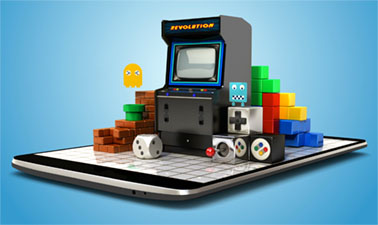
\includegraphics[width=\linewidth]{videoGame.jpg}
		\label{fig:videogame}
		\fonte{\citeonline{VideoGame2017}}
	\end{minipage}
	\hspace{0.2cm}
	\begin{minipage}[t]{0.45\linewidth}
		\centering
		\caption{Coxinha}
		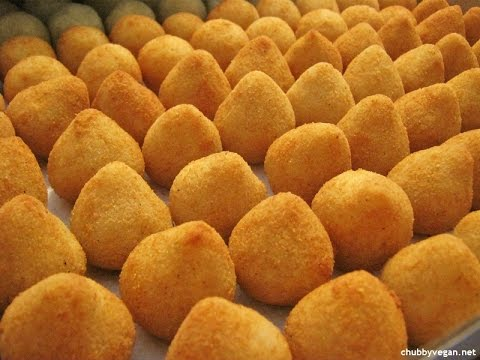
\includegraphics[width=0.8\linewidth]{coxinha.jpg}
		\label{fig:coxinha}
		\fonte{\citeonline{Coxinha2017}}
	\end{minipage}
\end{figure}

Na seção seguinte é apresentado exemplos de listas.


\section{Seção sobre Listas}

A seguir exemplos de 3 tipos de listas. Numerada, com bolinhas e com letrinhas.

\subsection{Lista Numerada}

A seguir exemplos de itens de lista numerada:

\begin{enumerate}[leftmargin=1.7cm]
	\item Sorvete;
	
	\item Coxinha;
	
	\item Pizza;
	
	\item Chocolate.
\end{enumerate}

\subsection{Lista com Bolinhas}

Exemplo de lista com marcadores circulares ou bolinhas:

\begin{itemize}[leftmargin=1.7cm]
	\item Sorvete;
	
	\item Coxinha;
	
	\item Pizza;
	
	\item Chocolate.
\end{itemize}

\subsection{Lista com Letrinhas}

Lista com identificadores com letras do alfabeto:

\begin{enumerate}[label=\alph*), leftmargin=1.7cm]
	
	\item Sorvete;
	
	\item Coxinha;
	
	\item Pizza;
	
	\item Chocolate.
	
\end{enumerate}

Na próxima seção são apresentados exemplos de textos itálicos, negritos e sublinhados.


\section{Textos}

Exemplos de textos \textit{itálicos}, \textbf{negrito} e \underline{sublinhado}:

Pra fazer texto itálico, a gente usa o comando \begin{verbatim} \textit{Palavra em Itálico} \end{verbatim}.

Pra fazer texto negrito, usamos o comando \begin{verbatim} \textbf{Palavra em Negrito} \end{verbatim}.

E para fazer um texto sublinhado, usamos \begin{verbatim} \underline{Palavra Sublinhada} \end{verbatim}.

A próxima seção apresenta exemplos de textos com notas de rodapé.

\section{Nota De Rodapé}

Para fazer uma nota de rodapé, usamos o comando \begin{verbatim} \footnote{Texto que vai no rodapé.} \end{verbatim}.

Aqui um exemplo de nota de rodapé\footnote{Essa é uma nota de rodapé.}.

As notas de rodapé também podem ter citações. O que problema nesse exemplo é que o texto, em um editor LaTeX pode ficar difícil de perceber e alterar\footnote{Essa é uma nota de rodapé que vai no meio do texto e ainda tem uma referência \cite{UTFPR2017}.}, mas ao gerar o PDF, ela fica mais perceptível.

A próxima seção apresenta exemplos de referências cruzadas.

\section{Referenciar Coisas Passadas}

Exemplos de como referenciar seções, imagens e tabelas que estão localizadas antes deste ponto do texto.

Para referenciar algo, é preciso que o que será referenciado tenha um \textit{label} e o local que referencia precisa usar um \textit{ref}.

Exemplo:

Aqui vamos referenciar a imagem do sorvete (Figura \ref{fig:sorvete}) que foi apresentada na seção \ref{sec:outra}.

Aqui vamos referenciar a tabela longa (Tabela \ref{tabela:longa}) que foi apresentada na seção \ref{sec:tabela}.


\section{Referenciar Coisas Futuras}

Também é possível referenciar conteúdos que ainda não foram apresentados, como é o caso desse exemplo que faz referência ao Apêndice (tabela \ref{tabela:tabelinha}), que é uma tabela simples, ou seja, não precisou de mais de uma página para ser apresentada.


% ----------------------------------------------------------
% ELEMENTOS PÓS-TEXTUAIS
% ----------------------------------------------------------
\postextual
% ----------------------------------------------------------
%
% ----------------------------------------------------------
% Referências bibliográficas
% ----------------------------------------------------------
\bibliography{referencias}


% ----------------------------------------------------------
% Apêndices
% ----------------------------------------------------------

% ---
% Inicia os apêndices
% ---
\ifthenelse{\equal{\ExisteApendice}{S}}
{
	\begin{apendicesenv}
	
	% Imprime uma página indicando o início dos apêndices
	\partapendices
	
	% ----------------------------------------------------------
\chapter{Tabela Tarefas}
% ----------------------------------------------------------

Texto de introdução, se necessário.

\begin{table}[H]
	\centering
	\caption{Tabelinha}
	\label{tabela:tabelinha}
	\begin{tabular}{lllllll}
		& \multicolumn{3}{l}{\textbf{Situação}} \\
		\hline                                % para uma linha horizontal
		
		\textbf{Atividades}                 & 1   & 2   & 3  \\
		\hline                                % para uma linha horizontal
		Ler  & \checkmark   & \checkmark   & \checkmark  \\
		Revisar &     & \checkmark   & \checkmark  \\
		Ajustar       & \checkmark   & \checkmark   & \checkmark  
	\end{tabular}
\end{table}
\fonte{Autoria própria}



	
	\end{apendicesenv}
}
% ---

% ----------------------------------------------------------
% Anexos
% ----------------------------------------------------------

% ---
% Inicia os anexos
% ---
\ifthenelse{\equal{\ExisteAnexo}{S}}
{
	\begin{anexosenv}
	
		% Imprime uma página indicando o início dos anexos
		\partanexos
	
		\chapter{Título do anexo 1}

Texto e informações do anexo.
	
	\end{anexosenv}
}
% ---

%---------------------------------------------------------------------
% INDICE REMISSIVO
%---------------------------------------------------------------------
\phantompart
\printindex
%---------------------------------------------------------------------

\end{document}
